\documentclass[a4paper,12pt]{article}         % класс документа - статья. Также report, book и др.
\usepackage{geometry}           % пакет для задания полей страницы командой \geometry
\geometry{left=3cm,right=1.5cm,top=2cm,bottom=2cm}
%\usepackage[cp1251]{inputenc}   % кодировка текста
\usepackage{mathtext}           % позволяет использовать русские буквы в формулах
\usepackage[T2A]{fontenc}       %пакет Т2А необходим для правильного отображения кириллицы и переноса слов
%\inputencoding{cp1251}          % тоже кодировка...
\usepackage[english,russian]{babel}      % языковой пакет - последний язык главный
%\usepackage[unicode]{hyperref}  %создаёт гиперссылки на список литературы в pdf-файле
\usepackage{amstext,amsmath,amssymb}            % пакеты для формул
\usepackage{bm}                 % boldmath - пакет для жирного шрифта
\usepackage[pdftex]{graphicx}   % пакет для включения рисунков в форматах png,pdf,jpg,mps,tif
                                % надо компилировать сразу в pdf
\usepackage{amsfonts}           % греческие символы и, возможно, что-то ещё
\usepackage{xcolor}
\usepackage{hyperref}
\usepackage{indentfirst}        % одинаковый отступ для первого параграфа и всего остального
\usepackage{cite}               % команда /cite{1,2,7,9} даёт ссылки
\usepackage{multirow}           % пакет для объединения строк в таблице: надо указать число строк и ширину столбца
\usepackage{array}              % нужен для создания таблиц
\usepackage{amsmath}
\linespread{1.3}                % полтора интервала. Если 1.6, то два интервала
\pagestyle{plain}               % номерует страницы
\definecolor{linkcolor}{HTML}{799B03} % цвет ссылок
\definecolor{urlcolor}{HTML}{799B03} % цвет гиперссылок

\hypersetup{pdfstartview=FitH,  linkcolor=linkcolor,urlcolor=urlcolor, colorlinks=true}
\bibliographystyle{gost780s}
\begin{document}
\begin{titlepage}
\begin{center}
Министерство науки и высшего образования РФ

ФГАОУ ВО Дальневосточный федеральный университет \flqq ДВФУ\frqq\\

Школа естественных наук\\
Кафедра компьютерных систем\\
\end{center}

\vspace{5cm}

\begin{center}
\LARGE \bf{Лабораторная работа №4}
\end{center}

\begin{center}\large
Разработка аппаратно-программного комплекса для ритмографии
\end{center}

\begin{center}\large
Диплом на соискание степени бакалавра
\end{center}

\vspace{3cm}

\large
\begin{flushright}
\textbf{Выполнил:}\\
студент группы Б8117-09.03.02\\
Мачехина Екатерина Владимировна\\

\vspace{1cm}

\textbf{Научный руководитель:}\\
(д.ф.-м.н.) \\
Плотников Владимир Сергеевич
\end{flushright}

\vspace{1cm}

\begin{center}
Владивосток 2021
\end{center}
\end{titlepage}

\tableofcontents

\newpage
\section{Примеры формул}
\paragraph{Алгоритм на основе дискретного преобразования Фурье}

В работе \cite{gothwal2011cardiac} был предложен алгоритм определения R - пиков QRS - комплекса с помощью дискретного преобразования Фурье - формула \ref{eq:sol1}.

\begin{equation}\label{eq:sol1}
x_{k}=\sum_{n=0}^{N-1}x_{n}e^{-2\pi jk\frac{n}{N}}, k = 0, ..., N-1
\end{equation}

На первом шаге работы алгоритмв из исходного электрокардиосигнала посредством прямого ДПФ формула \ref{eq:sol2} устраняются низкочастотные компоненты, приводящие к обнаружению ложных R - пиков. Далее выполняется восстановление сигнала с помощью обратного ДПФ.

\begin{equation}\label{eq:sol2}
C(\tau , s) = \frac{1}{\sqrt{\left |s  \right |}}\int_{-\infty }^{\infty }f(t)\Psi \left [ \frac{t-\tau}{s}  \right ]dt
\end{equation}


\begin{eqnarray}\label{eq:sol3}
J_\lambda(x_2, y_2, s_2) =
\iint K_\lambda(x_2, y_2) \cdot \Bigl| m_\lambda
\left(
\frac{x_2-x_0}{\lambda \cdot s_2} , \frac{y_2-y_0}{\lambda \cdot s_2}\right)\Bigr|^2 \,dx_0\,dy_0 = \nonumber \\
= K_\lambda(x_2, y_2) \otimes \Bigl| m_\lambda \left( \frac{x_2}{\lambda \cdot s_2} , \frac{y_2}{\lambda \cdot s_2} \right) \Bigr|^2
\end{eqnarray}

\newpage
\section{Примеры рисунков}

На рисунке \ref{fig:i1} показан принцип действия оптических датчиков пульса. Во время сердцебиения кровеносные сосуды то сужаются, то расширяются и из-за этого изменяется количество проходящей по ним крови, и соответственно и количество поглощаемого ею света.

\begin{figure}[h]
	\center{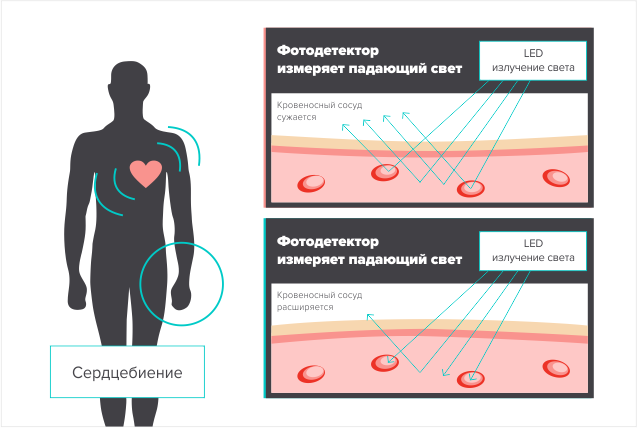
\includegraphics[scale=0.65]{1}}
	\caption{Принцип действия оптических датчиков пульса}
	\label{fig:i1}
\end{figure}

При спектральном анализе ВСР \ref{fig:i2} важное значение имеет длительность анализируемой выборки. При коротких записях (5 минут) выделяют три главных спектральных компоненты. Эти компоненты соответствуют диапазонам дыхательных волн и медленных волн 1-го и 2-го порядка. 

\begin{figure}[t]
	\center{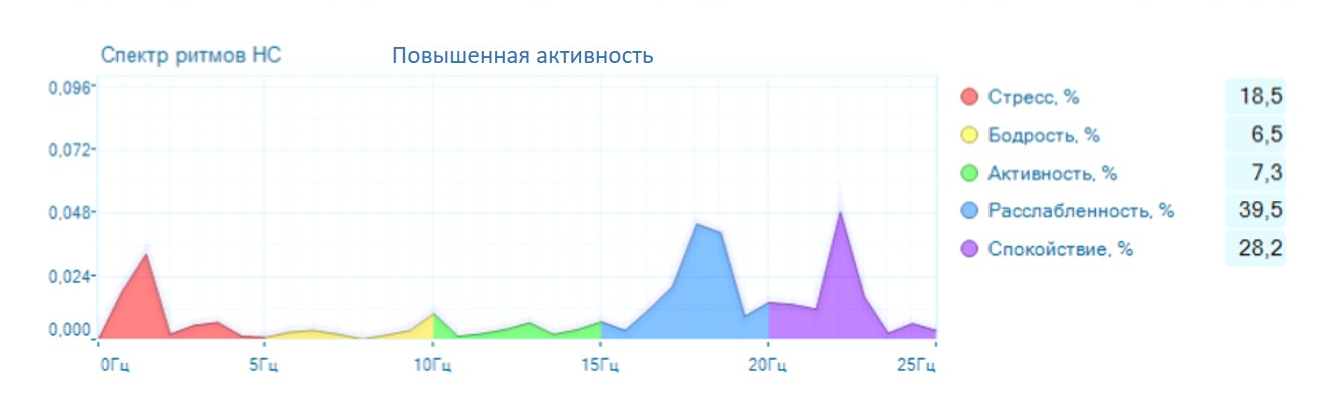
\includegraphics[scale=0.30]{2}}
	\caption{Спектральный анализ}
	\label{fig:i2}
\end{figure}

\paragraph{Непрерывное вейвлет - преобразование}
Вейвлет - преобразование одномерного сигнала состоит в его разложении по базису, основой которого выбрана некоторая порождающая функция (материнский вейвлет) - формула  \ref{eq:sol2}. Базис получают путём растяжения (сжатия) этой функции рисунок \ref{fig:i3}.

\begin{figure}[b]
	\center{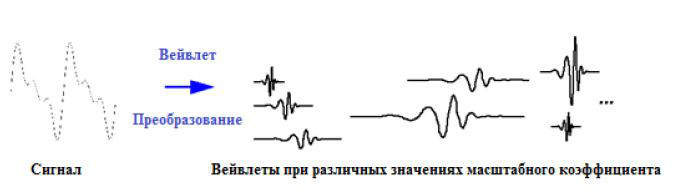
\includegraphics[scale=0.75]{3}}
	\caption{Формирование кардиоинтервалограммы}
	\label{fig:i3}
\end{figure}



\newpage
\section{Примеры таблиц}
\paragraph{Метод обработки продолжительных записей электрокардиосигналов} 
Метод обработки длительных записей строится на анализе вариабельности сердечного ритма. Основным объектом исследования являются ритмограммы, полученные из электрокардиограмм путём выделения QRS – комплексов. В зависимости от выбора метода определения ключевых параметров кардиограмм зависит точность дальнейшей обработки ЭКГ. В качестве используемого алгоритма обработки электрокардиограмм был выбран метод, основанный на непрерывном вейвлет – преобразовании, описанный в работе \cite{bolanos2006comparison} . 
По результатам проведённых исследования было установлено, что данный метод имеет достаточно высокую точность обнаружения QRS – комплексов, а также волн P и T, удовлетворяющую требованиям анализа Холтеровских записей. В таблице \ref{tabular:t1}  приведены результаты работы выбранного алгоритма на некоторых сигналах из базы данных MIT–BIH Normal Sinus Rhythm Database, предоставляемой в открытом доступе в сети интернет и содержащей записи длительностью не менее 25 часов.

\begin{table}[t]
\caption{\label{tabular:t1}Результаты работы алгоритма}
\begin{center}
	\begin{tabular}{|c|c|c|}
		\hline
		Номер сигнала & Se & P \\
		\hline
		16265 & 99,94  & 99,97\\
		16773 & 99,98  & 99,89 \\
		18177 & 99,97  & 99,91 \\
		19088 & 99,94  & 99,96 \\
		19830 & 99,96  & 99,92 \\
		\hline
		
	\end{tabular}
\end{center}
\end{table} 
Величина Se – способность алгоритма давать правильный результат, а P – вероятность фактического наличия характерной точки при положительном результате ее обнаружения.


\begin{table}[h]

	\caption{Сравнительный анализ алгоритмов}
	\label{tabular:t2}
	\begin{center}
		\begin{tabular}{|c|c|}
			\hline
			Название & Точность \\
			\hline
			Алгоритм Пана-Томпкинса & 98\\
			Корреляционный алгоритм & 94\\
			Алгоритм, основанный на подсчете числа пересечений нуля & 97,5\\
			Алгоритм на основе дискретного преобразования Фурье & 98\\
			Алгоритм на основе вейвлет - преобразования & 98,5\\
			\hline
		\end{tabular}
	\end{center}
\end{table}

Полученные из таблицы \ref{tabular:t2} результаты позволяют сделать вывод о том, что наиболее эффективные алгоритмы обнаружения QRS - комплексов строятся на основе нелинейных преобразований, разложения по базисным функциям, а также при использовании фильтрующих свойств оператора дифференцирования и интегрирования.

\newpage
\section{Gnuplot}
\begin{figure}[h]
	\centering
	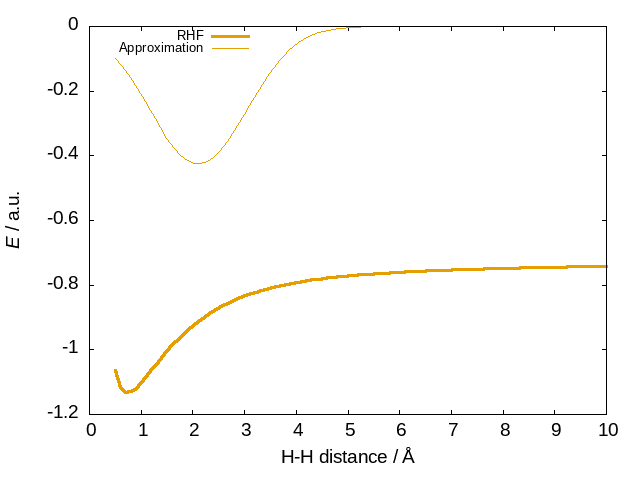
\includegraphics[width=0.8\linewidth]{plot.png}
	\smallskip
	\caption{Gnuplot: тестовые данные и их аппроксимация}
	\label{graph}
\end{figure}


\newpage
\bibliography{mybib}
\end{document}